\chapter{Resultados e Discussão}
\label{chap:resultados}

Analisar redes sociais permite vislumbrar as interações entre qualquer classe de indivíduos, partindo tanto de dados qualitativos quanto quantitativos. Segundo \cite{stanley1994social},  o uso de  análise de redes sociais possibilita coletar informações relevantes sobre a estrutura de um grupo, sendo possível, identificar as posições ocupadas pelos indivíduos, bem como identificar o cerne das relações criadas ao redor de cada um.

Como explicado anteriormente, os dados foram coletados no município de Icapuí-Ce, na \acrlong{UBS} da localidade de Barreira assim como em outros locais (Secretaria de Saúde do Município, o Centro de Atenção Psicossocial e o Hospital Municipal Maria Idalina Rodrigues de Medeiros), considerando as pessoas citadas nas entrevistas.

Logicamente, uma infinidade de análises pode ser realizada considerando os dados coletados, o que pode ser inviável de abordar em um único trabalho. Portanto, um número limitado de atores, conexões e métricas foi utilizado, e a partir deles, foram feitas considerações sobre o comportamento geral da rede social de uma única enfermeira. 

A rede pesquisada não contempla todas as relações possíveis e existentes de cada pessoa entrevistada, mas somente um recorte viável de analisar. As notações consideradas no desenho do grafo estão reunidas nas tabelas \ref{graph-job} e \ref{graph-place}.

\begin{table}[htbp]
\centering
\caption{Significado dos rótulos dos atores da rede segundo suas profissões.}
\label{graph-job}
\begin{tabular}{|l|l|}
\hline
Notação  & Profissão               \\ \hline
E        & Enfermeiro(a)           \\ \hline
E{[}R{]} & Enfermeiro(a) Residente \\ \hline
F        & Farmáceutico(a)         \\ \hline
N        & Nutricionista           \\ \hline
N{[}R{]} & Nutricionista Residente \\ \hline
M        & Médico(a)               \\ \hline
A        & Outro                   \\ \hline
\end{tabular}
\end{table}

\begin{table}[htbp]
\centering
\caption{Significado dos rótulos dos atores da rede segundo as áreas de atuação.}
\label{graph-place}
\begin{tabular}{|l|l|}
\hline
Notação & Área de Atuação                       \\ \hline
{[}H{]} & Hospital                      \\ \hline
{[}S{]} & Secretaria de Saúde de Icapuí \\ \hline
{[}P{]} & Policlínica de Aracati        \\ \hline
        & Atenção Básica                \\ \hline
\end{tabular}
\end{table}

Além disso, a identificação dos atores segue a seguinte notação [Profissão][Identificador Único] [Área de Atuação], por exemplo, $E1 [R]$ (Enfermeiro(a) 01 Residente); $E2$ (Enfermeiro 02 Atenção básica) etc.

Como pode ser observado na Figura \ref{fig:grafos}, o grafo permite identificar vinte e seis (26) atores que fazem parte da rede, onde seis (6) pessoas foram entrevistadas, vinte (20) outras foram citadas, trinta (30) relações e nenhum laço.

\begin{figure}[htbp]
\centering
 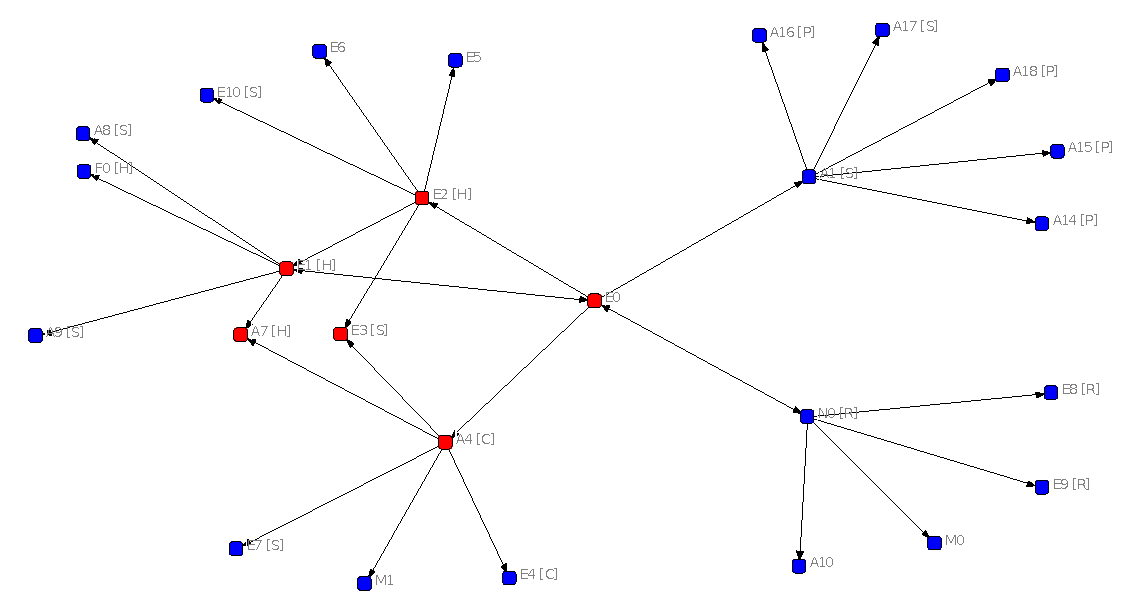
\includegraphics[width=.85\textwidth]{figuras/grafo-grupos.pdf}
 \caption{Representação da rede social utilizada neste trabalho.}
\label{fig:grafos}
\end{figure}

A primeira medida analisada da rede foi a densidade que é a relação entre o número de laços existentes e o número de laços possíveis. Tal métrica exibe a taxa de conectividade da rede. Neste trabalho, o valor de densidade encontrado foi de 4,61\% (baixa densidade) o que pode denotar a existência de alguma dificuldade na resolução de problemas em grupo.

Geralmente, nas circunstâncias onde existe baixa densidade, os atores não conseguem se identificar como participantes de um grupo maior e podem demonstrar certa dificuldade de relacionamento. Tal situação pode acarretar pouca cooperatividade entres os atores envolvidos, podendo até mesmo existir apatia na resolução de problemas, gerando conflitos. \cite{hanneman2001centralidad}.

Alexandra pode completar com a realidade que foi exibida com as entrevistas se contrapondo a ideia do parágrafo anterior.

Outra medida importante é o grau de centralidade, ele indica o número de ligações que entram e que saem de um ator. Através dele são identificados os atores principais da rede. A tabela \ref{table-centralize-degree} exibe o grau de centralidade associado a cada ator.

\begin{table}[htbp]
\centering
\caption{Grau de centralização de cada ator.}
\label{table-centralize-degree}
\begin{tabular}{|l|l|l|l|l|}
\hline
Identificador & Grau de Saída & Grau de Entrada & Grau de Saída  & Grau de Entrada \\ 
	      &               &                 & Normalizada    & Normalizada \\ \hline
E0            & 5,000         & 2,000           & 0,200                     & 0,080                       \\ \hline
A1 {[}S{]}    & 5,000         & 1,000           & 0,200                     & 0,040                       \\ \hline
E1 {[}H{]}    & 5,000         & 2,000           & 0,200                     & 0,080                       \\ \hline
N0 {[}R{]}    & 5,000         & 1,000           & 0,200                     & 0,040                       \\ \hline
A4 {[}C{]}    & 5,000         & 1,000           & 0,200                     & 0,040                       \\ \hline
E2 {[}H{]}    & 5,000         & 1,000           & 0,200                     & 0,040                       \\ \hline
F0 {[}H{]}    & 0,000         & 1,000           & 0,000                     & 0,040                       \\ \hline
A7 {[}H{]}    & 0,000         & 2,000           & 0,000                     & 0,080                       \\ \hline
A8 {[}S{]}    & 0,000         & 1,000           & 0,000                     & 0,040                       \\ \hline
A9 {[}S{]}    & 0,000         & 1,000           & 0,000                     & 0,040                       \\ \hline
A10           & 0,000         & 1,000           & 0,000                     & 0,040                       \\ \hline
E9 {[}R{]}    & 0,000         & 1,000           & 0,000                     & 0,040                       \\ \hline
E8 {[}R{]}    & 0,000         & 1,000           & 0,000                     & 0,040                       \\ \hline
M0            & 0,000         & 1,000           & 0,000                     & 0,040                       \\ \hline
A14 {[}P{]}   & 0,000         & 1,000           & 0,000                     & 0,040                       \\ \hline
A15 {[}P{]}   & 0,000         & 1,000           & 0,000                     & 0,040                       \\ \hline
A16 {[}P{]}   & 0,000         & 1,000           & 0,000                     & 0,040                       \\ \hline
A17 {[}S{]}   & 0,000         & 1,000           & 0,000                     & 0,040                       \\ \hline
A18 {[}P{]}   & 0,000         & 1,000           & 0,000                     & 0,040                       \\ \hline
E10 {[}S{]}   & 0,000         & 1,000           & 0,000                     & 0,040                       \\ \hline
E3 {[}S{]}    & 0,000         & 2,000           & 0,000                     & 0,080                       \\ \hline
E6            & 0,000         & 1,000           & 0,000                     & 0,040                       \\ \hline
E5            & 0,000         & 1,000           & 0,000                     & 0,040                       \\ \hline
E4 {[}C{]}    & 0,000         & 1,000           & 0,000                     & 0,040                       \\ \hline
M1            & 0,000         & 1,000           & 0,000                     & 0,040                       \\ \hline
E7 {[}S{]}    & 0,000         & 1,000           & 0,000                     & 0,040                       \\ \hline
\end{tabular}
\end{table}

Através da tabela \ref{table-centralize-degree} identifica-se que os principais atores da rede são $E0$, $E1[H]$, $A7 [H]$ e  $E3[S]$ pois cada um possui Grau de Entrada Normalizada de 0,8 (mais requisitados).

Alexandra pode falar sobre a importância dos principais atores da rede na resolução de problemas em icapuí.

O Grau de Proximidade denota a capacidade de um ator se ligar a todos os outros atores de uma rede, ou seja, quanto menor a distância entre um ator e outro, maior será seu grau de proximidade. 

Já o Grau de Intermediação mostra a capacidade que um ator possui de intermediar a comunicação entre pares de atores da rede. Sua importância se dá, pois, é através de atores que possuem alto grau de intermediação que as informações são propagadas para diversos outros atores. 

A tabela \ref{closeness-betweeness-degree} lista o Grau de Proximidade e Intermediação dos atores.

\begin{table}[htbp]
\centering
\caption{Grau de Proximidade e Intermediação dos Nós.}
\label{closeness-betweeness-degree}
\begin{tabular}{|l|l|l|}
\hline
Identificador & Grau de Proximidade & Grau de Intermediação \\ \hline
E0            & 55.556              & 66.667                \\ \hline
A1 {[}S{]}    & 42.373              & 36.667                \\ \hline
E1 {[}H{]}    & 44.643              & 26.333                \\ \hline
N0 {[}R{]}    & 40.984              & 30.000                \\ \hline
A4 {[}C{]}    & 42.373              & 27.333                \\ \hline
E2 {[}H{]}    & 44.643              & 26.333                \\ \hline
F0 {[}H{]}    & 31.250              & 0.000                 \\ \hline
A7 {[}H{]}    & 35.211              & 2.667                 \\ \hline
A8 {[}S{]}    & 31.250              & 0.000                 \\ \hline
A9 {[}S{]}    & 31.250              & 0.000                 \\ \hline
A10           & 29.412              & 0.000                 \\ \hline
E9 {[}R{]}    & 29.412              & 0.000                 \\ \hline
E8 {[}R{]}    & 29.412              & 0.000                 \\ \hline
M0            & 29.412              & 0.000                 \\ \hline
A14 {[}P{]}   & 30.120              & 0.000                 \\ \hline
A15 {[}P{]}   & 30.120              & 0.000                 \\ \hline
A16 {[}P{]}   & 30.120              & 0.000                 \\ \hline
A17 {[}S{]}   & 30.120              & 0.000                 \\ \hline
A18 {[}P{]}   & 30.120              & 0.000                 \\ \hline
E10 {[}S{]}   & 31.250              & 0.000                 \\ \hline
E3 {[}S{]}    & 35.211              & 2.667                 \\ \hline
E6            & 31.250              & 0.000                 \\ \hline
E5            & 31.250              & 0.000                 \\ \hline
E4 {[}C{]}    & 30.120              & 0.000                 \\ \hline
M1            & 30.120              & 0.000                 \\ \hline
E7 {[}S{]}    & 30.120              & 0.000                 \\ \hline
\end{tabular}
\end{table}

A partir da tabela \ref{closeness-betweeness-degree} observa-se que os atores $E0$, $A1 [S]$, $E1 [H]$, $N0 [R]$, $A4 [C]$ e $E2 [H]$ possuem os maiores Graus de Proximidade e os atores $E0$, $A1 [S]$ e $N0 [R]$ possuem maiores Graus de Intermediação.

Alexandra deve falar como os graus de intermediação e proximidade indicam bem a importância de A1 [S] da Central de Marcação de Consultas e exames.